\subsection{Strom/Spannnungsteiler}
    Spannungsteiler (Kondensator/Widerstand):\\
    \begin{minipage}{0.49\linewidth}
        \begin{center}
            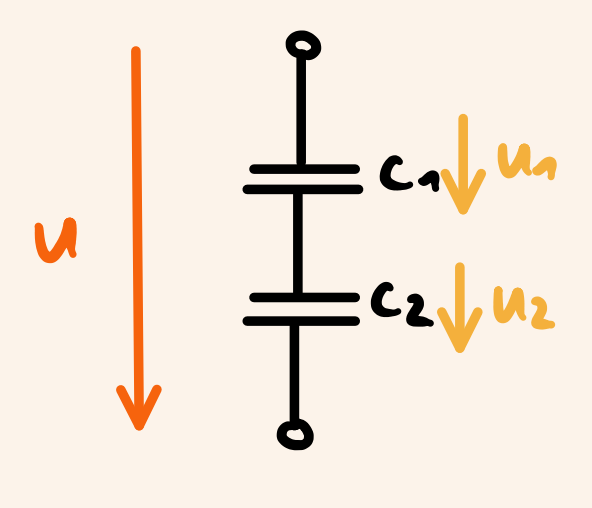
\includegraphics[width = 0.49\linewidth]{src/images/Spannungsteiler_1.png}
        \end{center}
    \end{minipage}
    \begin{minipage}{0.49\linewidth}
        \begin{center}
            \begin{empheq}[box=\fbox]{align*}
                U_1 = U \cdot \frac{C_1}{C_1 + C_2}\\
                U_2 = U \cdot \frac{C_2}{C_1 + C_2}
            \end{empheq}
        \end{center}
    \end{minipage}

    Stromteiler:\\
    \begin{minipage}{0.49\linewidth}
        \begin{center}
            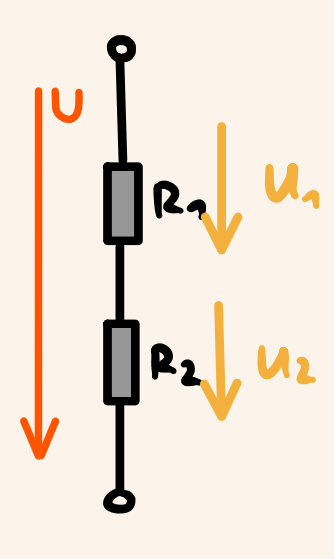
\includegraphics[width = 0.49\linewidth]{src/images/Spannungsteiler_2.png}
        \end{center}
    \end{minipage}
    \begin{minipage}{0.49\linewidth}
        \begin{center}
            \begin{empheq}[box=\fbox]{align*}
                I_1 = I \cdot \frac{R_1}{R_1 + R_2}\\
                I_2 = I \cdot \frac{R_2}{R_1 + R_2}
            \end{empheq}
        \end{center}
    \end{minipage}